\documentclass[
11pt, % The default document font size, options: 10pt, 11pt, 12pt
%codirector, % Uncomment to add a codirector to the title page
]{charter} 




% El títulos de la memoria, se usa en la carátula y se puede usar el cualquier lugar del documento con el comando \ttitle
\titulo{Visión por computadora para la identificación de flores y frutos de duraznero} 

% Nombre del posgrado, se usa en la carátula y se puede usar el cualquier lugar del documento con el comando \degreename
%\posgrado{Carrera de Especialización en Sistemas Embebidos} 
%\posgrado{Carrera de Especialización en Internet de las Cosas} 
\posgrado{Carrera de Especialización en Inteligencia Artificial}
%\posgrado{Maestría en Sistemas Embebidos} 
%\posgrado{Maestría en Internet de las cosas}

% Tu nombre, se puede usar el cualquier lugar del documento con el comando \authorname
\autor{Lic. Federico Lucas Paolino} 

% El nombre del director y co-director, se puede usar el cualquier lugar del documento con el comando \supname y \cosupname y \pertesupname y \pertecosupname
\director{Ing. Juan Ignacio Cavalieri}
\pertenenciaDirector{UNR} 
% FIXME:NO IMPLEMENTADO EL CODIRECTOR ni su pertenencia
\codirector{John Doe} % para que aparezca en la portada se debe descomentar la opción codirector en el documentclass
\pertenenciaCoDirector{FIUBA}

% Nombre del cliente, quien va a aprobar los resultados del proyecto, se puede usar con el comando \clientename y \empclientename
\cliente{Dr. Gerardo Sanchez}
\empresaCliente{INTA}


% Nombre y pertenencia de los jurados, se pueden usar el cualquier lugar del documento con el comando \jurunoname, \jurdosname y \jurtresname y \perteunoname, \pertedosname y \pertetresname.
\juradoUno{Nombre y Apellido (1)}
\pertenenciaJurUno{pertenencia (1)} 
\juradoDos{Nombre y Apellido (2)}
\pertenenciaJurDos{pertenencia (2)}
\juradoTres{Nombre y Apellido (3)}
\pertenenciaJurTres{pertenencia (3)}
 
\fechaINICIO{28 de febrero de 2023}		%Fecha de inicio de la cursada de GdP \fechaInicioName
\fechaFINALPlan{24 de abril de 2023} 	%Fecha de final de cursada de GdP
\fechaFINALTrabajo{octubre de 2023}	%Fecha de defensa pública del trabajo final


\begin{document}

\maketitle
\thispagestyle{empty}
\pagebreak


\thispagestyle{empty}
{\setlength{\parskip}{0pt}
\tableofcontents{}
}
\pagebreak


\section*{Registros de cambios}
\label{sec:registro}


\begin{table}[ht]
\label{tab:registro}
\centering
\begin{tabularx}{\linewidth}{@{}|c|X|c|@{}}
\hline
\rowcolor[HTML]{C0C0C0} 
Revisión & \multicolumn{1}{c|}{\cellcolor[HTML]{C0C0C0}Detalles de los cambios realizados} & Fecha      \\ \hline
0      & Creación del documento                                 &\fechaInicioName \\ \hline
1      & Se completa hasta el punto 5 inclusive                 & 14 de marzo de 2023 \\ \hline
2      & Se completa hasta el punto 9 inclusive                 & 21 de marzo de 2023 \\ \hline
3      & Se completa hasta el punto 12 inclusive                 & 28 de marzo de 2023 \\ \hline
%		  Se puede agregar algo más \newline
%		  En distintas líneas \newline
%		  Así                                                    & dd/mm/aaaa \\ \hline
%3      & Se completa hasta el punto 11 inclusive                & dd/mm/aaaa \\ \hline
%4      & Se completa el plan	                                 & dd/mm/aaaa \\ \hline
\end{tabularx}
\end{table}

\pagebreak



\section*{Acta de constitución del proyecto}
\label{sec:acta}

\begin{flushright}
Buenos Aires, \fechaInicioName
\end{flushright}

\vspace{2cm}

Por medio de la presente se acuerda con el \authorname\hspace{1px} que su Trabajo Final de la \degreename\hspace{1px} se titulará ``\ttitle'', el cual consistirá en la implementación de un detector y contador de frutos y flores de imágenes del duraznero, y tendrá un presupuesto preliminar estimado de 600 h de trabajo y \$1.850.000, con fecha de inicio el \fechaInicioName\hspace{1px} y fecha de presentación pública en \fechaFinalName.

Se adjunta a esta acta la planificación inicial.

\vfill

% Esta parte se construye sola con la información que hayan cargado en el preámbulo del documento y no debe modificarla
\begin{table}[ht]
\centering
\begin{tabular}{ccc}
\begin{tabular}[c]{@{}c@{}}Dr. Ing. Ariel Lutenberg \\ Director posgrado FIUBA\end{tabular} & \hspace{2cm} & \begin{tabular}[c]{@{}c@{}}\clientename \\ \empclientename \end{tabular} \vspace{2.5cm} \\ 
\multicolumn{3}{c}{\begin{tabular}[c]{@{}c@{}} \supname \\ Director del Trabajo Final\end{tabular}} \vspace{2.5cm} \\
%\begin{tabular}[c]{@{}c@{}}\jurunoname \\ Jurado del Trabajo Final\end{tabular}     &  & \begin{tabular}[c]{@{}c@{}}\jurdosname\\ Jurado del Trabajo Final\end{tabular}  \vspace{2.5cm}  \\
%\multicolumn{3}{c}{\begin{tabular}[c]{@{}c@{}} \jurtresname\\ Jurado del Trabajo Final\end{tabular}} \vspace{.5cm}                                                                     
\end{tabular}
\end{table}




\section{1. Descripción técnica-conceptual del proyecto a realizar}
\label{sec:descripcion}


\begin{consigna}{black} 
Contar de forma manual la cantidad de flores o frutos que posee un árbol a campo
resulta una tarea laboriosa. No obstante, conocer estos datos tiene diversas
aplicaciones que por su dificultad no están siendo abordadas. En el caso del departamento de biotecnología del INTA, los algoritmos a desarrollar se usaran como una herramienta interna del programa de mejoramiento. 

Automatizar la tarea de contar flores y frutos les permitirá obtener un gran volumen de datos para vincular con diferentes características, lo que se conoce como fenotipo, de interés como:
\begin{enumerate}
	\item Floribundidad: Relacionado con la tolerancia a heladas y producción.
	\item Fecha de floración plena: definir este estado fenológico de forma precisa
	\item Porcentaje de cuajado: Relacionado con la producción
	\item Potencial de raleo: capacidad de genotipo a soportar mayor o menor raleo.
	\item Rendimiento
\end{enumerate}

Actualmente no existen soluciones que permitan al cliente resolver el problema, tan solo existen papers e investigaciones de distintas universidades con temas similares. Esa es la razón por la cual el interesado decidió utilizar el programa de vinculación del laboratorio.

El objetivo de este proyecto consiste en contar con modelos de visión por computadora que permitan a los investigadores del área de biotecnología del INTA detectar y contar flores y frutos del duraznero. Actualmente es un tarea que se realiza de manera manual y requiere una gran cantidad de tiempo. El software resultante del proyecto permitirá a los investigadores ahorrar tiempo, simplemente deberán tomar fotografías de los arboles y el software se encargara de la detección y el conteo de elementos.

La principal valoración del cliente es que el entregable cumpla con el objetivo principal, que es hacer el recuento de estos elementos. No es requerimiento del cliente contar con una interfaz de usuario gráfica.

La gran mayoría de este tipo de proyectos pone el énfasis en detectar los elementos, pero no en contarlos, y si bien existen diferentes proyectos de detección de frutos, como también de flores, no se han encontrado proyectos que vinculen ambos y ademas hagan el recuento de los mismos.

La detección de objetos es una tarea importante en el campo de la visión por computadora y existen varios algoritmos que permiten hacerla, como los modelos de YOLO, RCNN, SSD, Resnet, etc. Todos estos modelos ya vienen con un pre-entrenamiento que permite adaptarlos al caso de uso del conteo de flores y frutos de los durazneros sin necesidad de un dataset de imágenes tan amplio ni tanto poder de cómputo. A la técnica de re-entrenar una red usando ya un previo entrenamiento se la conoce como \textit{transfer learning}.

El proceso resultante del presente trabajo contará con varias etapas, iniciando por la del etiquetado de las imágenes del dataset, continuara por hacer la aumentación de datos (\textit{data augmentation}), un proceso por el cual se le aplican diferentes filtros a las imágenes para agrandar el dataset. Una vez realizado este proceso,  se entrenarán los diferentes modelos con el dataset extendido y se probará la eficiencia de cada uno. 

En la Figura \ref{fig:diagBloques} se presenta el diagrama en bloques del sistema. En este se puede observar que una vez realizado el entrenamiento de los diferentes modelos deberemos realzar el ajuste fino (\textit{fine tunning}), un proceso por el cual editamos los hiper-parámetros del entrenamiento de las redes para que brinde los mejores resultados con el escenario actual.

\begin{figure}[htpb]
\centering 
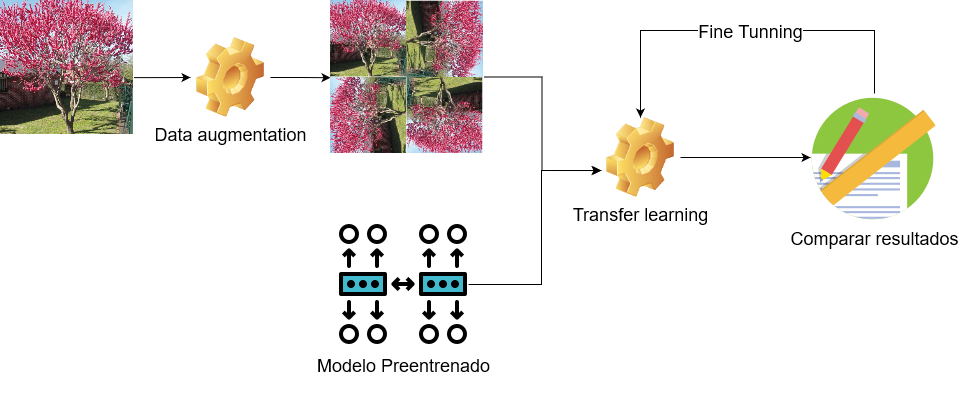
\includegraphics[width=0.80\textwidth]{./Figuras/Diagrama entrenamiento.png}
\caption{Diagrama en bloques del sistema}
\label{fig:diagBloques}
\end{figure}

\vspace{25px}


\end{consigna}

\section{2. Identificación y análisis de los interesados}
\label{sec:interesados}


\begin{table}[ht]
%\caption{Identificación de los interesados}
%\label{tab:interesados}
\begin{tabularx}{\linewidth}{@{}|l|X|X|l|@{}}
\hline
\rowcolor[HTML]{C0C0C0} 
Rol           & Nombre y Apellido & Organización 	& Puesto 	\\ \hline
Auspiciante   &                   & INTA             	&        	\\ \hline
Cliente       & \clientename      &\empclientename	& Investigador en Biotecnología        	\\ \hline
Responsable   & \authorname       & FIUBA        	& Alumno 	\\ \hline
Orientador    & \supname	      & \pertesupname 	& Director Trabajo final \\ \hline
\end{tabularx}
\end{table}



\section{3. Propósito del proyecto}
\label{sec:proposito}

\begin{consigna}{black}
El propósito de este proyecto es crear un programa que permita a los miembros del área de biotecnología del INTA detectar y contar tanto frutos como flores del duraznero a partir de diferentes imágenes.
\end{consigna}

\section{4. Alcance del proyecto}
\label{sec:alcance}

\begin{consigna}{black}
El presente proyecto incluye la entrega del código fuente para el modelo de visión por computadora y toda la documentación necesaria para poder ejecutar este mismo.

El proyecto no incluye soporte visual (interfaz de usuario) ni software donde se implemente el código. La ejecución del modelo queda a cargo del usuario final.
\end{consigna}


\section{5. Supuestos del proyecto}
\label{sec:supuestos}

\begin{consigna}{black}
Para el desarrollo del presente proyecto se supone que: 

\begin{itemize}
	\item Se tiene la disponibilidad de al menos 600 horas para la realización del proyecto.
	\item El tiempo estimado es suficiente para realización del proyecto.
	\item Al momento de finalizar la cursada de las materias del posgrado se tendrá el conocimiento suficiente para poder realizar el proyecto.
	\item Se puede acceder al dataset para realizar el proyecto.
	\item Las imágenes del dataset cuentan con una resolución mínima de 640x640.
	\item Se tienen mas de 500 imágenes de cada categoría (frutos y flores).
	\item La detección de los elementos no deberá ser precisa al 100\%, se establecerá un umbral de aceptación.
	\item Se tiene una GPU con al menos 8 gigabytes de VRAM en la cual entrenar los modelos. 
\end{itemize}
\end{consigna}

\section{6. Requerimientos}
\label{sec:requerimientos}

\begin{consigna}{black}
Los requerimientos deben numerarse y de ser posible estar agruparlos por afinidad, por ejemplo:

\begin{enumerate}
	\item Requerimientos funcionales
		\begin{enumerate}
			\item El software debe identificar los frutos y flores del duraznero con una precision superior al umbral definido.
			\item El software debe contar por separado frutos y flores.
		\end{enumerate}
	\item Requerimientos de documentación
		\begin{enumerate}
			\item El software sera entregado con un manual de uso.
			\item Al finalizar el desarrollo se entregara un informe de precision.
			\item El código del software debe estar desarrollado de forma prolija y siguiendo las practicas sugeridas por los docentes de la carrera.
			
		\end{enumerate}
	\item Requerimientos de testing
		\begin{enumerate}
			\item Una vez finalizado el proyecto se realizaran pruebas con nuevas fotos tomadas por los investigadores.
			\item Los resultados entregados por el software deberán ser aprobados por los investigadores.
		\end{enumerate}
		
\end{enumerate}

\end{consigna}

\section{7. Historias de usuarios (\textit{Product backlog})}
\label{sec:backlog}
\begin{consigna}{black}
Primero y principal, se especifica la forma para puntuar cada historia. Los criterios
son:
\begin{enumerate}
	\item Dificultad: La cantidad de trabajo a realizar
	\item Complejidad: El nivel de sofisticación del trabajo
	\item Riesgo: El nivel de riesgo que involucra realizar la tarea
\end{enumerate}

Los números disponibles a la hora de puntuar cada categoría son aquellos definidos en la sucesión de Fibonacci, yendo de 1 a 8. Cada una de las historia tendrá su puntaje por categoría y después para calcular el total de los puntos se sumaran las 3 categorías.

Una vez que realicemos la suma, la secuencia se puede extender hasta el 34.


Historia 1:
Como investigador quiero poder detectar las flores y frutos del duraznero para poder ingresar la información en el sistema de fenotipos
\begin{enumerate}
	\item Dificultad: 8, la tarea incluye etiquetado, el aumento de los datos y la corrida de los modelos.
	\item Complejidad: 5, Se necesitan conocimientos avanzados en algoritmia y visión por computadora.
	\item Riesgo: 8, esta tarea es clave de todo el desarrollo, sin esta no se puede continuar con las demás.
	\item Total: 34
\end{enumerate}


Historia 2 (depende de historia 1):
Como investigador quiero poder contar las flores y frutos del duraznero una vez detectado para poder ingresar la información en el sistema de fenotipos
\begin{enumerate}
	\item Dificultad: 2, es algo que ya se ha realizado en bastas oportunidades.
	\item Complejidad: 3, se necesita conocimiento de algoritmia intermedios.
	\item Riesgo: 3, si bien la tarea es importante, la realización es corta y se puede modificar fácilmente.
	\item Total: 8
\end{enumerate}

Historia 3 (depende de historia 1):
Como investigador quiero poder saber cual es la confianza que se tiene de la detección de los elementos para poder definir si los datos son lo suficientemente aceptables para el sistema de fenotipos
\begin{enumerate}
	\item Dificultad: 2, es algo que ya se ha realizado en bastas oportunidades.
	\item Complejidad: 3, se necesita conocimiento de algoritmia intermedios.
	\item Riesgo: 1, la precision ya debería haber sido establecida en las pruebas finales.
	\item Total: 8
\end{enumerate}

\end{consigna}

\section{8. Entregables principales del proyecto}
\label{sec:entregables}

\begin{consigna}{black}

Los entregables del proyecto son:

\begin{itemize}
	\item Manual de uso.
	\item Código fuente.
	\item Informe final.
	\item Informe de precision.
	\item Dataset aumentado y etiquetado.
\end{itemize}

\end{consigna}

\section{9. Desglose del trabajo en tareas}
\label{sec:wbs}
\begin{consigna}{black}
\begin{enumerate}
\item Planificación (62 hs)
	\begin{enumerate}
	\item Definir alcance (6 hs)
	\item Definir director (8 hs)
	\item Redactar planificación (48 hs)
	\end{enumerate}
\item Etiquetado y aumento de datos (80 hs)
	\begin{enumerate}
	\item Etiquetado (40 hs)
	\item Investigación de técnicas de aumentación de datos (8 hs)
	\item Aplicación de data aumentación de datos (32 hs)
	\end{enumerate}
\item Aprendizaje transferido (296 hs)
	\begin{enumerate}
	\item Investigación de modelos de visión por computadora (24 hs)
	\item Implementación y entrenamiento del primer modelo (20 hs)
	\item Ajuste fino del primer modelo (40 hs)
	\item Implementación y entrenamiento del segundo modelo (20 hs)
	\item Ajuste fino del segundo modelo (40 hs)
	\item Implementación y entrenamiento del tercer modelo (20 hs)
	\item Ajuste fino del tercer modelo (40 hs)
	\item Implementación y entrenamiento del cuarto modelo (20 hs)
	\item Ajuste fino del cuarto modelo (40 hs)
	\item Crear software final (32 hs)
	\end{enumerate}
\item Testing (48 hs)
	\begin{enumerate}
	\item Evaluar y decidir mejor modelo junto con usuario final (12 hs)
	\item Pruebas de comportamiento del software final (8 hs)
	\item Pruebas con nuevas imágenes del cliente (8 hs)
	\item Pruebas de velocidad de inferencia(6 hs)
	\item Pruebas de precision de inferencia(6 hs)
	\item Pruebas en vivo con el cliente (8 hs)
	\end{enumerate}
\item Documentación (118 hs)
	\begin{enumerate}
	\item Redactar memoria técnica (96 hs)
	\item Redactar manual de usuario (6 hs)
	\item Redactar informe de precision (6 hs)
	\item Redactar informe de avance (10 hs)
	\end{enumerate}
\end{enumerate}

Cantidad total de horas: 604 hs.


\end{consigna}

\section{10. Diagrama de Activity On Node}
\label{sec:AoN}

\begin{consigna}{black}

En la Figura \ref{fig:AoN} se detallan las referencias de diagrama de Activity on Node.

En la Figura \ref{fig:AoN2} se detalla el diagrama de Activity on Node.

%La figura \ref{fig:AoN} fue elaborada con el paquete latex tikz y pueden consultar la siguiente referencia \textit{online}:

%\url{https://www.overleaf.com/learn/latex/LaTeX_Graphics_using_TikZ:_A_Tutorial_for_Beginners_(Part_3)\%E2\%80\%94Creating_Flowcharts}

\end{consigna}

\begin{figure}[htpb]
\centering 
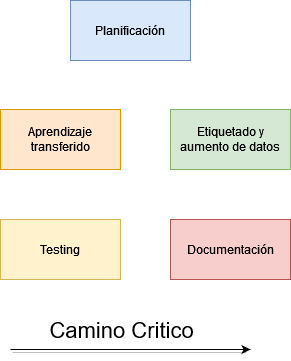
\includegraphics[width=.45\textwidth]{./Figuras/Aon referencias.png}
\caption{Referencias Diagrama de \textit{Activity on Node}.}
\label{fig:AoN}
\end{figure}

\begin{figure}[htpb]
\centering 
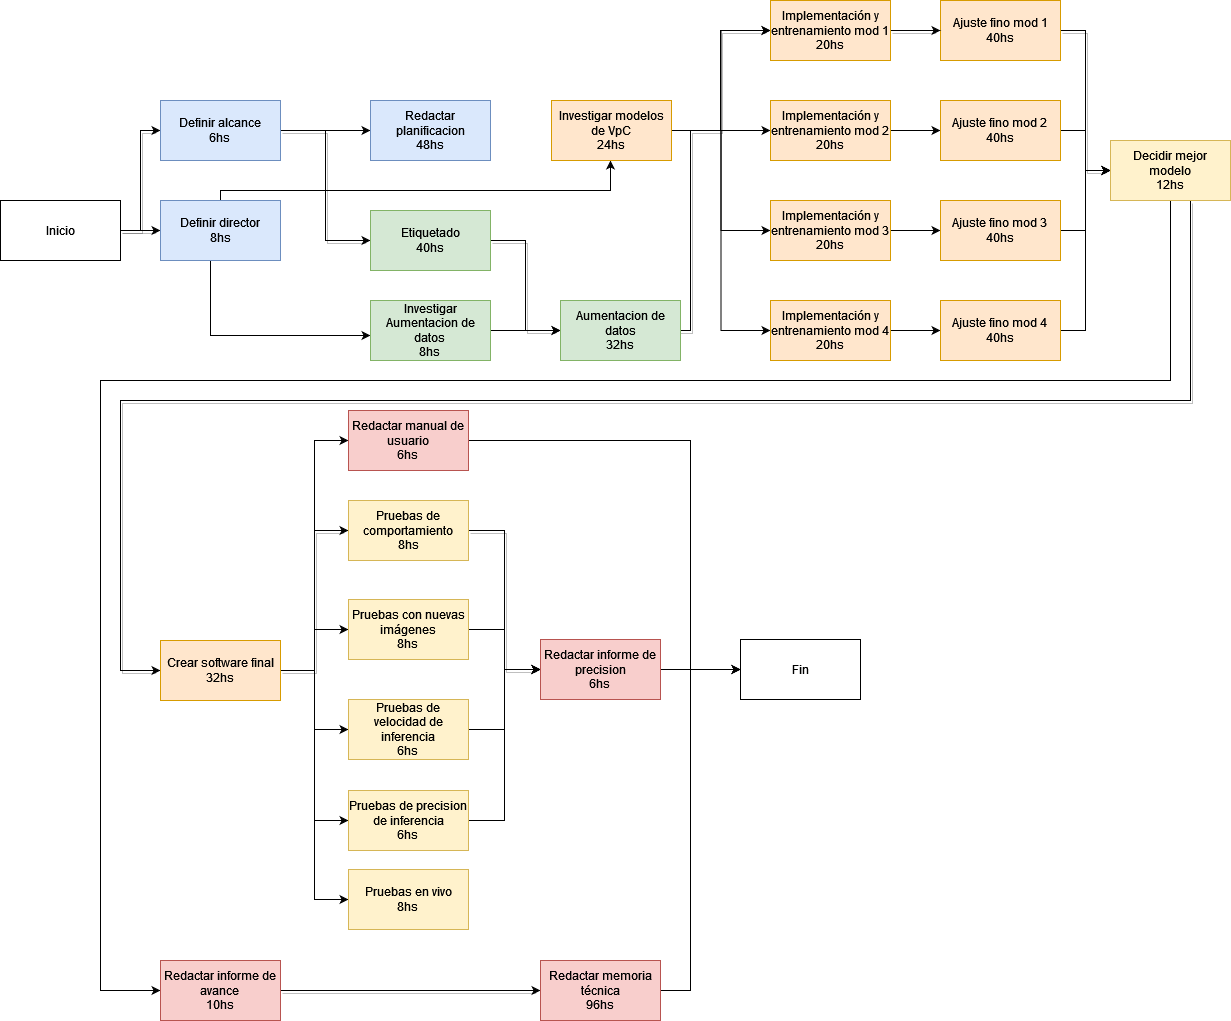
\includegraphics[width=.99\textwidth]{./Figuras/AoN finalv2.png}
\caption{Diagrama de \textit{Activity on Node}.}
\label{fig:AoN2}
\end{figure}


\section{11. Diagrama de Gantt}
\label{sec:gantt}

\begin{consigna}{black}

\begin{landscape}
\vspace*{50px}

\begin{figure}[htpb]
\centering 
\begin{center}
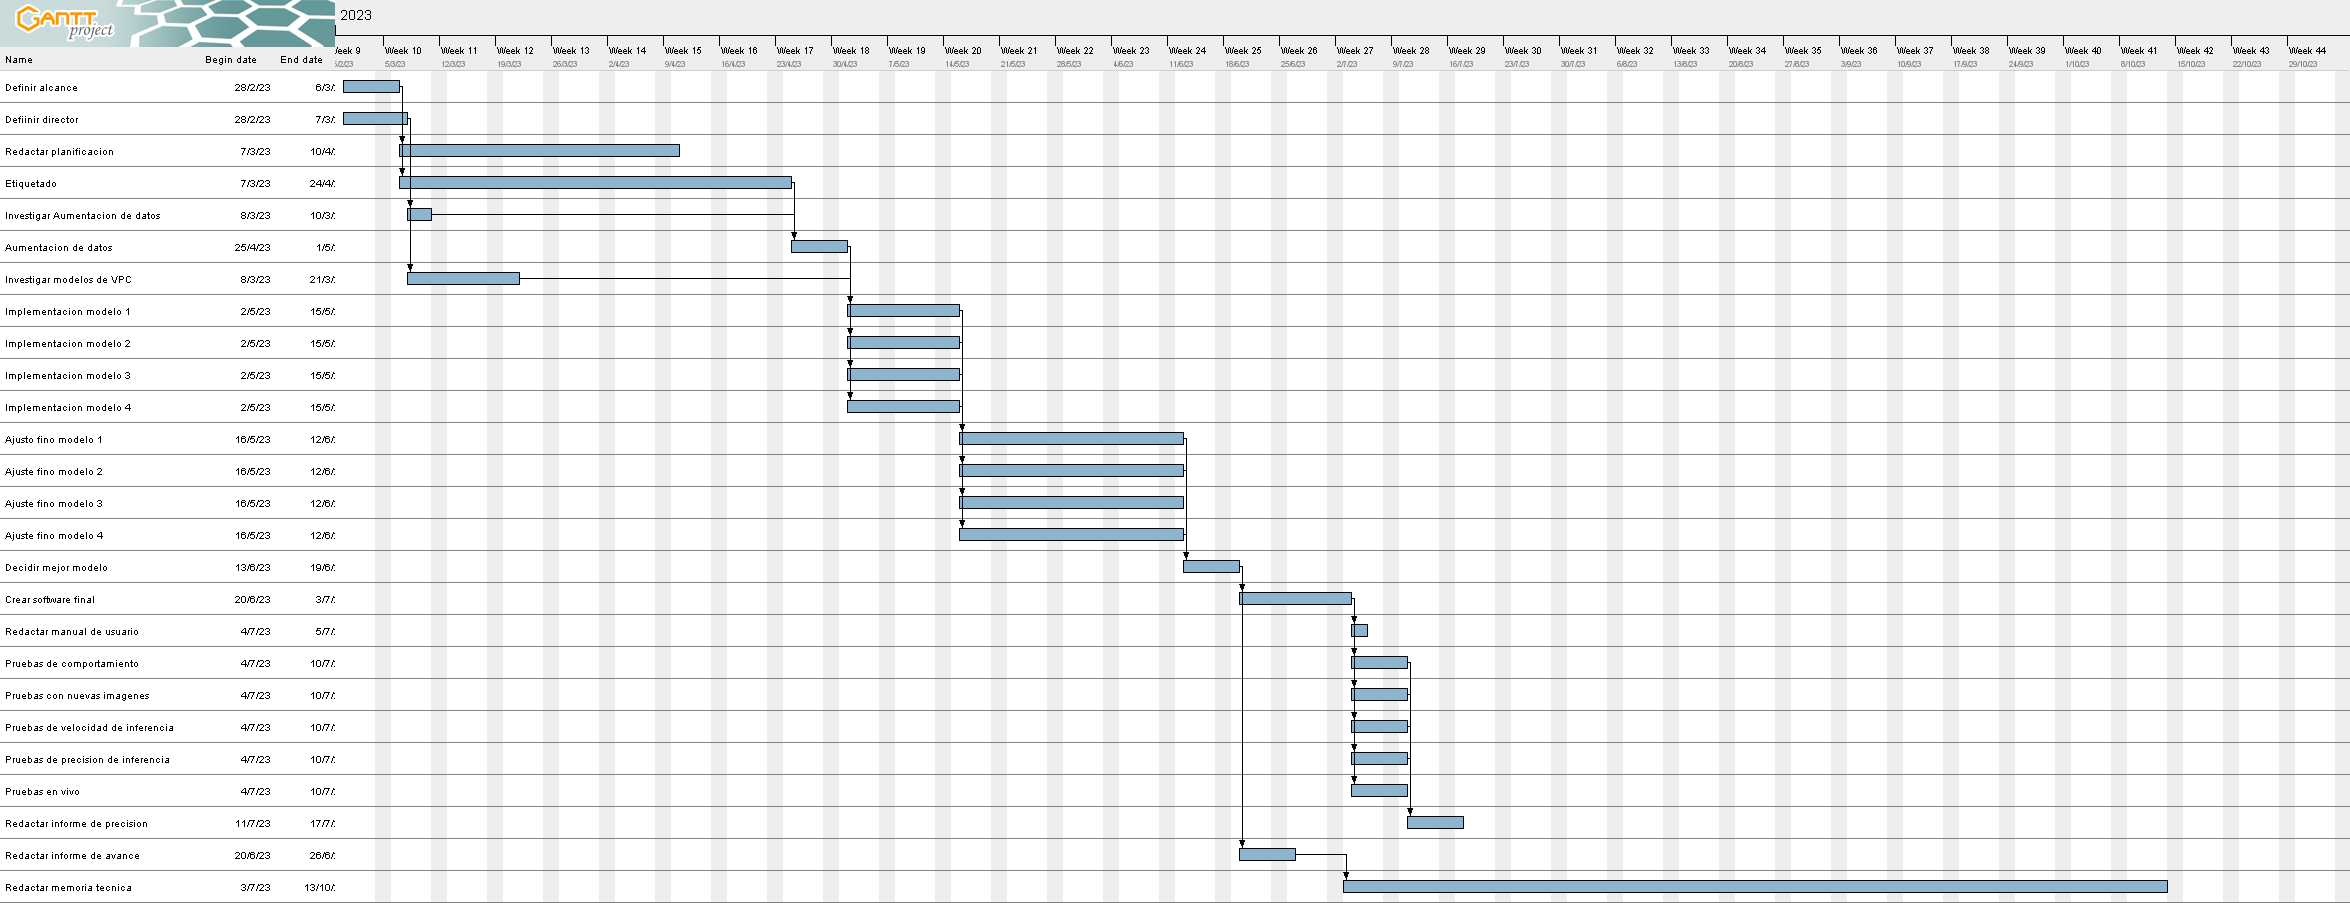
\includegraphics[height=.6\textwidth]{./Figuras/Untitled Project 4.png}
\caption{Diagrama de \textit{Gantt}.}
\label{fig:Gantt}
\end{center}
\end{figure}
\end{landscape}


\end{consigna}


\section{12. Presupuesto detallado del proyecto}
\label{sec:presupuesto}

\begin{consigna}{black}

\end{consigna}

\begin{table}[htpb]
\centering
\begin{tabularx}{\linewidth}{@{}|X|c|r|r|@{}}
\hline
\rowcolor[HTML]{C0C0C0} 
\multicolumn{4}{|c|}{\cellcolor[HTML]{C0C0C0}COSTOS DIRECTOS} \\ \hline
\rowcolor[HTML]{C0C0C0} 
Descripción &
  \multicolumn{1}{c|}{\cellcolor[HTML]{C0C0C0}Cantidad} &
  \multicolumn{1}{c|}{\cellcolor[HTML]{C0C0C0}Valor unitario} &
  \multicolumn{1}{c|}{\cellcolor[HTML]{C0C0C0}Valor total} \\ \hline
Mano de obra & 
  \multicolumn{1}{c|}{604} &
  \multicolumn{1}{c|}{\$2500} &
  \multicolumn{1}{c|}{\$1510000} \\ \hline

\multicolumn{3}{|c|}{SUBTOTAL} &
  \multicolumn{1}{c|}{\$1510000} \\ \hline
\rowcolor[HTML]{C0C0C0} 
\multicolumn{4}{|c|}{\cellcolor[HTML]{C0C0C0}COSTOS INDIRECTOS} \\ \hline
\rowcolor[HTML]{C0C0C0} 
Descripción &
  \multicolumn{1}{c|}{\cellcolor[HTML]{C0C0C0}Cantidad} &
  \multicolumn{1}{c|}{\cellcolor[HTML]{C0C0C0}Valor unitario} &
  \multicolumn{1}{c|}{\cellcolor[HTML]{C0C0C0}Valor total} \\ \hline
Internet & 
  \multicolumn{1}{c|}{8} &
  \multicolumn{1}{c|}{\$2000} &
  \multicolumn{1}{c|}{\$16000} \\ \hline
Consumo electrico & 
  \multicolumn{1}{c|}{8} &
  \multicolumn{1}{c|}{\$3000} &
  \multicolumn{1}{c|}{\$24000} \\ \hline
GPU NVIDIA 24Gb de RAM & 
  \multicolumn{1}{c|}{1} &
  \multicolumn{1}{c|}{\$300000} &
  \multicolumn{1}{c|}{\$300000} \\ \hline
\multicolumn{3}{|c|}{SUBTOTAL} &
  \multicolumn{1}{c|}{\$340000} \\ \hline
\rowcolor[HTML]{C0C0C0}
\multicolumn{3}{|c|}{TOTAL} &
	\multicolumn{1}{c|}{\$1850000} \\ \hline
\end{tabularx}%
\end{table}


\section{13. Gestión de riesgos}
\label{sec:riesgos}

\begin{consigna}{red}
a) Identificación de los riesgos (al menos cinco) y estimación de sus consecuencias:
 
Riesgo 1: detallar el riesgo (riesgo es algo que si ocurre altera los planes previstos de forma negativa)
\begin{itemize}
	\item Severidad (S): mientras más severo, más alto es el número (usar números del 1 al 10).\\
	Justificar el motivo por el cual se asigna determinado número de severidad (S).
	\item Probabilidad de ocurrencia (O): mientras más probable, más alto es el número (usar del 1 al 10).\\
	Justificar el motivo por el cual se asigna determinado número de (O). 
\end{itemize}   

Riesgo 2:
\begin{itemize}
	\item Severidad (S): 
	\item Ocurrencia (O):
\end{itemize}

Riesgo 3:
\begin{itemize}
	\item Severidad (S): 
	\item Ocurrencia (O):
\end{itemize}


b) Tabla de gestión de riesgos:      (El RPN se calcula como RPN=SxO)

\begin{table}[htpb]
\centering
\begin{tabularx}{\linewidth}{@{}|X|c|c|c|c|c|c|@{}}
\hline
\rowcolor[HTML]{C0C0C0} 
Riesgo & S & O & RPN & S* & O* & RPN* \\ \hline
       &   &   &     &    &    &      \\ \hline
       &   &   &     &    &    &      \\ \hline
       &   &   &     &    &    &      \\ \hline
       &   &   &     &    &    &      \\ \hline
       &   &   &     &    &    &      \\ \hline
\end{tabularx}%
\end{table}

Criterio adoptado: 
Se tomarán medidas de mitigación en los riesgos cuyos números de RPN sean mayores a...

Nota: los valores marcados con (*) en la tabla corresponden luego de haber aplicado la mitigación.

c) Plan de mitigación de los riesgos que originalmente excedían el RPN máximo establecido:
 
Riesgo 1: plan de mitigación (si por el RPN fuera necesario elaborar un plan de mitigación).
  Nueva asignación de S y O, con su respectiva justificación:
  - Severidad (S): mientras más severo, más alto es el número (usar números del 1 al 10).
          Justificar el motivo por el cual se asigna determinado número de severidad (S).
  - Probabilidad de ocurrencia (O): mientras más probable, más alto es el número (usar del 1 al 10).
          Justificar el motivo por el cual se asigna determinado número de (O).

Riesgo 2: plan de mitigación (si por el RPN fuera necesario elaborar un plan de mitigación).
 
Riesgo 3: plan de mitigación (si por el RPN fuera necesario elaborar un plan de mitigación).

\end{consigna}


\section{14. Gestión de la calidad}
\label{sec:calidad}

\begin{consigna}{red}
Para cada uno de los requerimientos del proyecto indique:
\begin{itemize} 
\item Req \#1: copiar acá el requerimiento.

\begin{itemize}
	\item Verificación para confirmar si se cumplió con lo requerido antes de mostrar el sistema al cliente. Detallar 
	\item Validación con el cliente para confirmar que está de acuerdo en que se cumplió con lo requerido. Detallar  
\end{itemize}

\end{itemize}

Tener en cuenta que en este contexto se pueden mencionar simulaciones, cálculos, revisión de hojas de datos, consulta con expertos, mediciones, etc.  Las acciones de verificación suelen considerar al entregable como ``caja blanca'', es decir se conoce en profundidad su funcionamiento interno.  En cambio, las acciones de validación suelen considerar al entregable como ``caja negra'', es decir, que no se conocen los detalles de su funcionamiento interno.

\end{consigna}

\section{15. Procesos de cierre}    
\label{sec:cierre}

\begin{consigna}{red}
Establecer las pautas de trabajo para realizar una reunión final de evaluación del proyecto, tal que contemple las siguientes actividades:

\begin{itemize}
	\item Pautas de trabajo que se seguirán para analizar si se respetó el Plan de Proyecto original:
	 - Indicar quién se ocupará de hacer esto y cuál será el procedimiento a aplicar. 
	\item Identificación de las técnicas y procedimientos útiles e inútiles que se emplearon, y los problemas que surgieron y cómo se solucionaron:
	 - Indicar quién se ocupará de hacer esto y cuál será el procedimiento para dejar registro.
	\item Indicar quién organizará el acto de agradecimiento a todos los interesados, y en especial al equipo de trabajo y colaboradores:
	  - Indicar esto y quién financiará los gastos correspondientes.
\end{itemize}

\end{consigna}


\end{document}
